\documentclass[a4paper, 11pt]{scrartcl}

% font, language
\usepackage[utf8]{inputenc}
\usepackage[T1]{fontenc}
\usepackage{lmodern}

\usepackage{float}
\usepackage{longtable}

% quoting
\usepackage{quoting, xparse}
\usepackage[hyphens]{url}

\usepackage[toc,page]{appendix}

% highliting
\usepackage{color,soul}

\NewDocumentCommand{\bywhom}{m}{% the Bourbaki trick
  {\nobreak\hfill\penalty50\hskip1em\null\nobreak
   \hfill\mbox{\normalfont(#1)}%
   \parfillskip=0pt \finalhyphendemerits=0 \par}%
}

\NewDocumentEnvironment{pquotation}{m}
  {\begin{quoting}[
     indentfirst=true,
     leftmargin=\parindent,
     rightmargin=\parindent]\itshape}
  {\bywhom{#1}\end{quoting}}

\usepackage{todonotes}
\usepackage{caption}
\newcommand{\source}[1]{\caption*{\hfill Source: {#1}} }

\usepackage{fontspec}
\setmainfont{Latin Modern Roman}

\usepackage{polyglossia}
\setmainlanguage[babelshorthands=true]{german}
\setdefaultlanguage[spelling=new]{german}
\usepackage[autostyle]{csquotes}
\MakeAutoQuote{»}{«}



% graphics
\usepackage{graphicx}
\graphicspath{ {images/} }

% code highlighting
\usepackage{listings}
\usepackage{color}
\lstset{ % General setup for the package
	language=java
}

% toc depth
\setcounter{tocdepth}{4}
\setcounter{secnumdepth}{4}

% bib
\usepackage[
	backend=biber,
	sorting=none
]{biblatex}

\addbibresource{references/references.bib}
\usepackage{hyperref}
\usepackage{xcolor}
\hypersetup{
	colorlinks,
	linkcolor={red!0!black},
	citecolor={blue!70!black},
	urlcolor={blue!70!black}
}

\usepackage{enumitem}
\setlist[enumerate]{label*=\arabic*.}

% title, author
\title{Bachelor-Thesis}
\author{Roman Quistler}

\begin{document}
	
	% \begin{titlepage}
	\centering
	
\includegraphics[width=0.30\textwidth]{hsb_logo.png}
	\par\vspace{1cm}
	{\scshape\LARGE Hochschule Bremen \par}
	\vspace{1cm}
	{\scshape\Large Bachelorarbeit  \par}
	\vspace{1.5cm}
	{\LARGE\bfseries Entwicklung eines Model-View-Intent Framework für die Plattform Android\par}
	\vspace{0.5cm}
	{\normalsize\itshape Medieninformatik B.Sc. \par}
	\vspace{2cm}
	{\Large\itshape Roman Quistler \par}
	\vfill
	\vfill
	{\large\today\par}
\end{titlepage}
	
	\pagenumbering{gobble}
	\newpage
	\tableofcontents
	\newpage
	\pagenumbering{arabic}
	
	\newpage
	
	\section{Einleitung}
\label{sec:einleitung}

Bis zum Jahre 1973 und der Entwicklung des ersten Eingabegerätes mit Graphischer Oberfläche (GUI) (Xerox Alto \cite{xeroxAlto}) erfolgte die Interaktion mit einem Computer im Wesentlichen über eine Konsole. Dies reduzierte die Ein- und Ausgabe eines Programms auf rein textuelle Elemente. Seither hat sich viel getan: Die Erschaffung des Internets leitet den Beginn von Webseiten ein, welche von einer anfänglich statischen Ausprägung zu der heutigen dynamisch und komplexen wuchsen. Dazu gesellten sich im Laufe der Zeit mobile Endgeräte - zu Beginn bestückt mit Tasten für die Eingabe, sowie einem primitiven Bildschirm für die Anzeige finden sich heutzutage vorwiegend leistungsfähige, auf einem kapazitiven Touchscreen basierende Smartphones wieder. Hierbei ist über die Jahre der Funktionsumfang von Betriebssystem und Applikationen im Allgemeinen gestiegen.

\subsection{Problemfeld}
\label{subsec:problemfeld}
Die Herausforderung für einen Entwickler ist es, die Nutzerschnittstelle (auch: »Presenation Layer« \cite{presentationLayerpatternsOfEnterpriseApplicationArchitectureMartinFowler}),
innerhalb einer »Drei-Schichtenarchitektur«
\cite{threeTierArchitectureDonaldWolfe2013}
sinnvoll aufzubauen und dabei die Modellierung und Verwaltung des Zustandes innerhalb einer Applikation zu berücksichtigen. Hierfür müssen auch externe Vorkommnisse wie bspw.. die Aktualisierung der zugrundeliegenden Datenbank miteinbezogen werden.
\\\\
Da diese Problematik nicht erst seit kurzem sondern seit vielen Jahren besteht, wurden hierfür bereits unterschiedliche Ansätze entwickelt. Diese spiegeln sich in sogenannten Architekturmuster wieder und bieten ein Mittel, den »Presentation Layer« sinnvoll zu organisieren.
\\\\
Zu diesen Architekturmuster hat sich im Jahre 2015 ein neues hinzugesellt: »Model-View-Intent (MVI)«. Es besitzt bereits bekannte Herangehensweisen, setzt jedoch auch auf neue Ideen. Zu Beginn kam es ausschließlich in der Entwicklung von Webanwendungen zum Einsatz, bis es mit etwas Verzögerung auch in der (nativen) Android Entwicklung Einzug hielt. Wie es meist der Fall ist wenn neue Wege beschritten werden, ergibt sich viel Ungeklärtes. Dieses wächst wenn zusätzlich eine Wechsel der Plattform vorgenommenen, welche trotz Gemeinsamkeiten erhebliche Unterschiede und aufweist.
\\\\
Ist ein Entwickler an einem Einsatz von MVI interessiert, so ergeben sie für ihn gewisse, wenn auch übliche Hindernisse: Wie lassen sie die jeweiligen Komponenten umsetzten? Wie gut lassen sich Implementierungen für eine Plattform auf eine andere, seine Übertragen? Inwieweit müssen Eigenheit beachtet werden?  

\subsection{Ziel der Arbeit}
\label{subsec:ziel-der-arbeit}
Mit der Arbeit wird das Ziel verfolgt, das Architekturmuster MVI zu untersuchen, besser zu verstehen und im Kontext Android ein Framework zu schaffen.
\\
Es sollen Eigenheiten der Plattform, sowie allgemeine Probleme ausgemacht werden die für den Einsatz von MVI in Android relevant sind. Dazu müssen bereits bestehende Lösung evaluiert und vorhandene Problematiken aufgezeigt werden. Auf Basis der gewonnenen Erkenntnisse soll daraufhin ein kleines und dogmatisches Framework entwickelt werden. Die Absicht ist dem Anwender alle nötigen Komponenten zu Realisierung von MVI zur Verfügung zu stellen und eine klare Struktur vorzugeben. Dabei soll der Aufwand seitens des Nutzers möglichst gering gehalten werden.

\subsection{Aufbau der Arbeit}
\label{subsec:aufbau-der-arbeit}
Im ersten Schritt werden die nötigen Grundlagen für ein besserer Verständnis von MVI geklärt. Dazu gehören spezielle Paradigmen der Programmierung als auch vorausgegangene Konzepte und Bibliotheken.
\\\\
Ist dies Vollbracht so wird im nächsten Schritt MVI mit all seinen Komponenten genau beschrieben. Es wird auch versucht, die Gründe für die Entstehung von MVI zu finden und zu erläutern.
\\\\
Daraufhin werden die Funktionalen und Nichtfunktionalen Anforderung für das zu entwickelnde Framework aufgelistet und näher ausgeführt. Hierbei soll Erkennbar ein, worauf der Fokus liegt und was als Optional eingestuft wird. 
\\\\
Im weiteren Fortgang wird mit diesen Anforderung und den zuvor erworbenen Kenntnissen das Framework und seine individuellen Komponenten konzipiert. Jeder dieser wird ausführlich beleuchtet und ihre Funktion dargelegt. Auch die Zusammenhänge innerhalb des Frameworks werden aufgegriffen und erörtert.
\\\\
Anschließend erfolgt die Implementation des Framework in Form eines Prototypen. Zuvor werden jedoch Grundlegende Entscheidungen und ihre Auswirkungen erläutert. 
\\\\
Als vorletzter Schritt werden die jeweiligen Anforderungen auf Basis des Prototypen ausgewertet. Es wird geschaut zu welchem Grad diese Erfüllt wurden und falls nicht, welche Gründe dies hat und wie es umgesetzt werden könnte. Außerdem sollen eventuelle Verbesserungen diskutiert werden.
\\\\
Zum Schluss wird die Arbeit und ihr Ergebnis zusammengefasst und ein Ausblick gegeben.

	\newpage
	
	\section{Grundlagen}
\label{sec:grundlagen}

In diesem Kapitel gilt es zu klären, auf welchen Grundlagen, Ideen und Konzepten Model-View-Intent beruht, wie diese miteinander fungieren und weshalb sie als Inspiration dienten.

\subsection{Unidirektionaler Datenfluss und der Zustand: Flux, Redux und Elm}

In einer Applikation existieren grundsätzlich zwei Komponenten: Eine, die der Nutzer wahrnehmen kann und eine, die für ihn unsichtbar bleibt. Bei ersterer handelt es sich meist um das, was der Nutzer(auf dem Bildschirm) sieht - die sogenannte »View«. Die zweite Komponente beschreibt die Ebene, welche das Geschehen observiert, darauf reagiert und den weiteren Verlauft (zum größten Teil) kontrolliert. Sie kann unter anderem als »Controller« betitelt werden.
\\
\\
Ein weiterer, essentieller Aspekt einer Anwendung ist ihr Zustand. Dieser kann sich aus mehreren Teilen zusammensetzten:
\begin{itemize}
	\item Alles was der Nutzer sieht
	\item Daten die über das Netzwerk geladen werden
	\item Standort des Nutzer
	\item Fehler die auftreten
	\item \dots
\end{itemize}
Der Zustand in dem sich eine Applikation befindet kann hierbei von beiden Seiten modifiziert und beobachtet werden. Ist dies der Fall, so handelt es sich um einen bidirektionalen Datenfluss. Bei dieser Variante entsteht die eventuelle Gefahr von kaskadierenden Updates (ein Objekt verändert ein anderes, welches wiederum eine Veränderung bei einem weiteren herbeiführt usw.) als auch in einen unvorhersehbaren Datenfluss zu geraten: Es wird schwer, den Fluss der Daten nachzuvollziehen. Des weiteren muss immer überprüft und sichergestellt werden, dass »View« und »Controller« synchronisiert sind, da beide den globalen Zustand darstellen. Schlussendlich verliert man zusätzlich die Fähigkeit zu entscheiden, wann und and welcher Stelle der Zustand manipuliert wird.
\\
\\
Ein anderer Ansatz ist, den Datenfluss in eine Richtung zu beschränken und ihn damit unidirektional
\cite{unidirectionalDataFlowFluxArchitectureIlyGelman2017, unidirectionalDataFlowTheCompleteReduxBookIlyGelman2017}
operieren zu lassen. Diese Variante erfreut sich an zunehmender Popularität seit der Bekanntmachung der »Flux«
\cite{fluxArchitectureAdamBoduch}
Architektur im Jahre 2015 von Facebook.
\cite{fluxAnnouncementYoutube}

\subsubsection{Flux}
Für die Einhaltung und Umsetzung eines unidirektionalen Datenfluss und der Verwaltung des Zustands bedient sich »Flux« bei zwei fundamentalen Konzepten: Der Zustand innerhalb einer Applikation wird als »single source of truth (SSOT)« angesehen und darf keine direkte Änderung erfahren. Um dies zu Gewährleisten finden sich mehrere Komponenten in »Flux« wieder:
\\
\\
\textbf{Action}: Eine Aktion beschreibt ein Ereignis, welches unter anderem vom Nutzer ausgelöst werden kann. Sie geben vor, wie mit der Anwendung interagiert wird. Jeder dieser Aktionen wird dabei ein Typ zugewiesen. Insgesamt sollte eine Aktion semantisch und deskriptiv bezüglich der Intention sein. Des weiteren können zusätzliche Attribute an eine Aktion gebunden werden.
\\
\begin{lstlisting}[frame=single, language=Java]
{
 type: ActionTypes.INCREMENT,
 by: 2
}
\end{lstlisting}
\bigskip
\textbf{Dispatcher}: Er ist für die Entgegennahme und Verteilung einer Aktion an sogenannte »Stores« zuständig. Diese haben die Möglichkeit sich beim ihm zu registrieren. Er besitzt die wichtige Eigenschaft der sequentiellen Verarbeitung, d.h., dass er zu jedem Zeitpunkt nur eine »Action« weiterreicht. Sämtliche »Stores« werden über alle Aktionen unterrichtet.
\\
\\
\textbf{Store}: Hier befinden sich die Daten, welche einen Teil des globalen Zustands einer Anwendung ausmachen. Die einzige Möglichkeit für eine Veränderung der dort hinterlegten Daten besteht durch ein Reaktion auf eine, vom »Dispatcher« kommenden, Aktion. Bei jeder Modifikation der Daten erfolgt die Aussendung eines Events an eine »View«, das die Veränderung mitteilt.
Ebenso findet sich hier ein Part der Anwendungslogik.
\\
\\
\textbf{View}: Die View ist für die Anzeige und Eingabe von Daten zuständig - sie ist die für den Nutzer sichtbare Komponente, mit welcher dieser interagiert. Ihre Daten erhält sie von einem »Store«, diesen sie abonniert und auf Änderungsereignisse hört. Erhält sie vom »Store« ein solches Änderungsereignis, so kann sie die neuen Daten abrufen und sich selbst aktualisieren. Der View ist es nicht gestattet, den Zustand direkt zu verändern. Stattdessen generiert sie eine Aktion schickt diese an den Dispatcher.
\\
Ein Beispielhafter Ablauf bei einer Anwendung die einen Wert erhöht oder verringert kann wie folgt aussehen:
\begin{enumerate}
	\item Die View bekommt einem Store zugewiesen, welcher für das inkre- und dekrementieren der angezeigten Zahl verantwortlich ist.
	\item Sie erhält die Anfangszahl und stellt diese in einem leserlichen Format/einer Ansicht dar, welches es dem Nutzer ermöglicht, damit zu interagieren.
	\item Betätigt dieser einer der Knöpfe welche die dargestellte Zahl verändern, so wird eine Action erstellt und an Dispatcher geschickt.
	\item Dieser wiederum informiert alle Stores.Information
	\item Jener Store der für die Verarbeitung dieser Aktion verantwortlich ist, modifiziert die Zahl in seiner internen Datenstruktur und kommuniziert dies über ein Änderungsereignis
	\item Diejenige View, welche auf Änderungsereignisse diesen Ursprungs lauscht, erhält die Daten und aktualisiert sich dementsprechend. 
\end{enumerate}

\begin{figure}[ht]
	\centering
	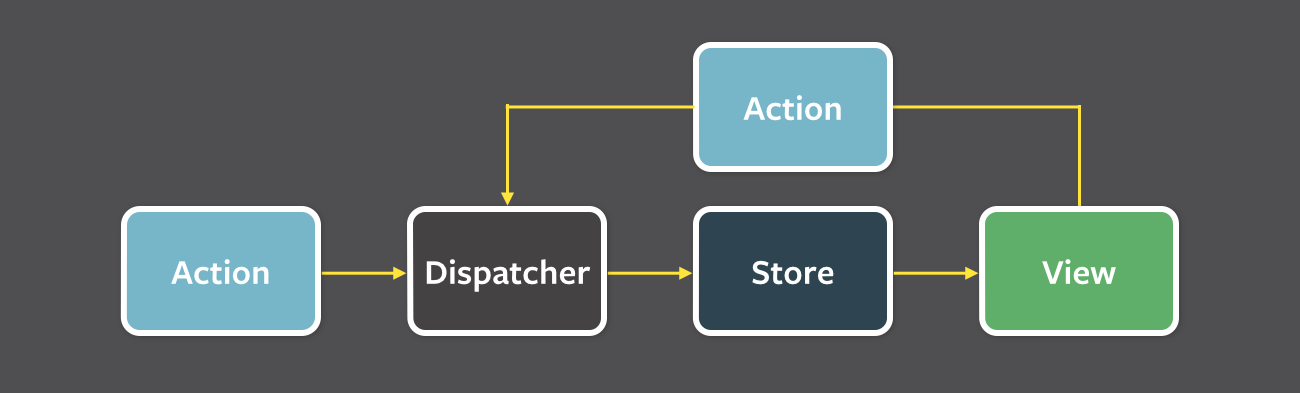
\includegraphics[height=0.25\textwidth]{./images/flux-flow}
	\caption{Datenfluss in der Flux Architektur}
	\label{fig:datenflussFlux}
\end{figure}

Anhand Abbildung \ref{fig:datenflussFlux} wird der unidirektionale Datenfluss deutlich erkennbar:
\begin{enumerate}
	\item Die View schickt eine Aktion an den Dispatcher.
	\item Dieser leitet diese an alle Stores weiter.
	\item Der Store verarbeitet die Daten und informiert die View.
\end{enumerate}
\bigskip
Insgesamt liefert Flux mit diesen Komponenten eine Möglichkeit, einen unidirektionalen Fluss herzustellen und die Verwaltung des Zustands einer Applikation zu vereinfachen.
\subsubsection{Redux}
Bei Redux handelt sich um eine JavaScript Bibliothek (und kein Framework) welche ihre Inspiration aus Flux und Elm bezieht. Sie wurde im Jahre 2015 von Dan Abramov und Andrew Clark ins Leben gerufen.
\cite{reduxIntroduction}
Auch hier nimm der direktionale Datenfluss eine wesentliche Rolle ein.
\\
\\
Die Bibliothek kann als eine vereinfachte Form von Flux verstanden werden, welche gewisse Elemente und Ansätze übernimmt, aber auch streicht bzw. ersetzt. Genau wie Flux existieren die bereits behandelten Actions, welche über wichtige Informationen für die spätere Veränderung des Zustands verfügen. Auch hier können diese ihren Ursprung in einer vom Nutzer getätigten Aktion haben. Wird eine Aktion ausgeführt, so spricht man von einer Versendung einer Aktion. Dieser Versand findet nur dann statt, wenn man die Intention verfolgt, den Zustand zu ändern. Sie gelangt zu einem sogenannten "Reducer". Hier findet sich der erste Grundlegende Unterschied zu Flux.
\\
\\
Ein "Reducer" ist für sich genommen eine einfache Funktion, die bei gleicher Eingabe die immer gleiche Ausgabe erzeugt. Sie ist dabei frei von sogenannten Seiteneffekten und wird als "pure" bezeichnet. Im Falle eines "Reducers" erwartet dieser die vorher erzeugte Aktion und den globalen, derzeitigen Zustand der Anwendung. Sein Aufgabe ist es, aus der Kombination dieser einen neuen Zustand zu generieren. Hierfür wird die Aktion, basierend auf ihrem Typ und eventuellen Inhalt, ausgewertet und der Zustand dementsprechend angepasst. Dabei ist zu beachten, dass keine direkte Manipulation des Zustands möglich ist, stattdessen wird ein komplett neuer Zustand zurückgegeben. Diese Eigenschaft der Unveränderbarkeit wird gemeinhin als "Immutability" erfasst.
\\
\begin{lstlisting}[frame=single, language=Java]
(previousState, action) => newState
\end{lstlisting}
\ \\
Das Verbindungsstück zwischen einer Aktion und dem Reducer bildet der Store. Dieser existiert im Gegensatz zu Flux nur ein einziges Mal (und mit auch der Zustand) und ist für die Verwaltung des Zustands verantwortlich. Er übernimmt zugleich auch die Rolle des Dispatchers, wie er in Flux vorkommt, und verteilt die Akionen an alle Reducer weiter. Der aus dem diesen Prozess hervorgehende, neue Zustand wird im Store hinterlegt. Dieses Ereignis wird ebenfalls seitens der View observiert, welche im Anschluss die nötigen Aktualisierungen an der Ansicht vornimmt.
Am Ende lässt sich der gesamte Fluss wie folgt darstellen:
\\
\begin{lstlisting}[frame=single, language=Java]
View -> Action -> Reducer(s) -> Store -> View
\end{lstlisting}
\bigskip
Neben Redux existieren in der JavaScript Welt noch weitere Bibliotheken, die entweder eine Abwandlungen von Flux darstellen oder aber neue Konzepte implementieren. Jedoch verfolgen dabei alle eine ähnliches Ziel: Ein unidirektionaler Datenfluss und die (zentrierte) Verwaltung des Zustands einer Anwendung.

\subsubsection{Elm}
Bei Flux und Redux handelt es sich jeweils um Bibliotheken die innerhalb einer Anwendung verwendet werden können. Eine weitere Herangehensweise ist die Verankerung solcher Konzepte in der Programmiersprache selbst. Dies findet man z.B. in
der Programmiersprache Elm
\cite{elmIntroduction}
wieder. Elm besitze eine in die Sprache integrierte Architektur die den einfach Namen "The Elm Architecture" 
\cite{theElmArchitecture}
trägt. Eine andere Variante lautet: Model-View-Update. Anhand dessen lassen sich bereits die Kern-Komponenten der Entwurfsmusters erahnen.
\\
\\
\textbf{Model:} Das Model repräsentiert den Zustand der Applikation als eine simple Datenstruktur.
\\
\textbf{View:} Die View ist eine Funktion, welche aus einem Model HTML code generiert. Ebenfalls wie in Flux wird kommt auch hier das Konzept von "pure functions" zum tragen: Die gleiche Eingabe erzeugt die gleich Ausgabe - ohne Ausnahme.
\subsection{Funktionale Programmierung}
Im Verlaufe der Kapitel wurden bereits Begriffe wie eine "reine" Funktion (pure functions) oder die Unveränderlichkeit (Immutibilty) einen Datenstruktur angesprochen. Diese Konzepte zählen zu einem Programmierparadigma, welches in den letzten Jahren auch an Bedeutung in Sprachen wie Java gewonnen hat
\cite{javaFunctionalProgramming}
: Funktionale Programmierung.
\\
\\
In der häufig imperativen, Objektorientierte Programmierung wie sie in Java oder auch C\# anzutreffen ist, machen Klassen und
die Mutation (in möglicher Abhängigkeit von gewissen Konditionen) solcher den Hauptbestandteil des Quellcodes aus. Dabei ist zu beachten, dass die funktionale Programmierung die Objektorientierte nicht zwingenden ausschließt, sondern lediglich in eingeschränkter Form nutzt.
Eine Implementierung in Java welche Beispielweise den Name eines Nutzer Objekts ändert, könnte wie folgt aussehen:
\begin{lstlisting}[frame=single, language=Java]
public User changeUserName(String newUserName, User currentUser){
 if(newUserName != null){
  currentUser.name = newName
		
  System.out.println("Changed user name to: " + newUserName)	
 }
	
 return currentUser
}
\end{lstlisting}

	
	\newpage
	
	\begin{appendix}
		\listoffigures
	\end{appendix}

	\printbibliography[type=book,title={Book References}]

	\printbibliography[type=report,title={Report References}]
	
	\printbibliography[type=article,title={Artikel Referenzen}]
	
	\printbibliography[type=thesis,title={Thesis References}]
	
	\printbibliography[type=online,title={Online References}]
	
\end{document}
